\chapter{深度学习相关技术}\label{chap:dl}
基于深度学习的乳腺钼靶分类问题本质上是传统的计算机视觉分类检测问题。为此,本文应用了卷积神经网络对乳腺钼靶数据进行特征提取,基于目前最成熟的两阶段模型Faster R-CNN对乳腺钼靶病灶进行定位分析。考虑到数据量少、训练不易收敛等问题,迁移在传统大数据集上训练好的模型到医疗影像数据进行学习;同时考虑到部分数据未标注,引入弱监督学习的方法,并为了充分挖掘模型区分正常样本和恶性样本的能力,考虑使用度量学习。为此,本文所考虑到的所有的深度学习技术将在本章具体介绍。
\section{卷积神经网络}
深度学习以数据作为输入,经过算法抽象将数据变为最终任务需要的高维特征,完成特征到任务之间的映射。其中,代表算法是神经网络算法,包括深度置信网络、递归神经网络和卷积神经网络等。特别是CNN,目前在计算机视觉、医疗影像处理等领域发挥着重要的作用,这个也是本文主要涉及到的关键技术。

CNN是特殊的人工神经网络,区别于神经网络其他模型(如递归神经网络,Boltzmann机等)。卷积神经网络是一种带有卷积结构的深度神经网络,卷积结构可以减少深层网络占用的内存量,其存在三个关键的操作,第一是局部感受野,第二是权值共享,第三是通过pooling层有效地减少网络的参数个数,缓解了模型的过拟合问题。CNN在众多领域应用尤其是图像相关任务表现优异,诸如图像分类、图像语义分割、物体检测等计算机视觉问题。另外,随着研究的深入,如自然语言处理中的文本分类、软件工程数据挖掘中的软件缺陷预测等问题都在尝试利用卷积神经网络解决,并取得了相比传统方法甚至其他深度网络模型更有的预测结果。

CNN发展历史中的第一件关键时间是上世纪60年代左右的神经科学中,加拿大神经科学家David H.hubel于1959年提出猫的初级视皮层中单个神经元的"感受野"概念,在1962年发现猫的视觉中枢里存在感受野、双目视觉等其他功能结构,标志着神经网络结构首次在大脑视觉系统中被发现\cite{38Ba2013Do}。

随后,Yann LeCun等人在1998年提出基于梯度学习的CNN算法\cite{39lecun1998gradient},并将其成功用于手写数字字符识别。他们提出的LeNet模型\ref{fig:dl_lenet}是第一个产生实际商业价值的卷积神经网络,同时也为卷积神经网络以后的发展奠定了坚实的基础。 
\begin{figure}[!htbp]
    \centering
    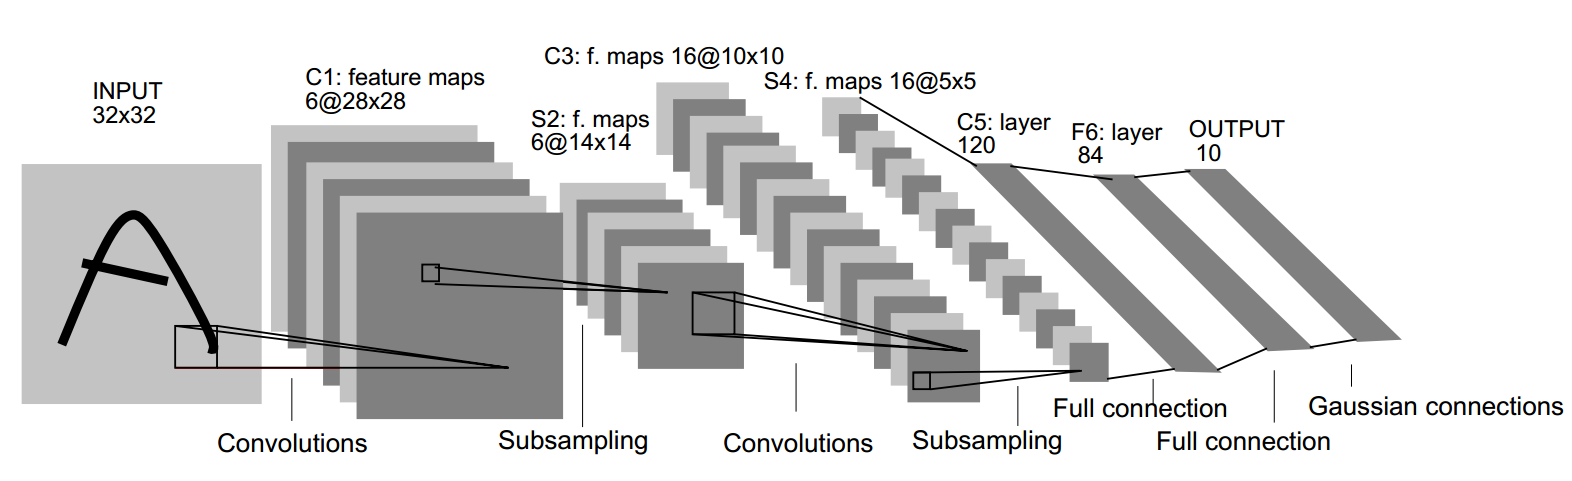
\includegraphics[width=0.7\textwidth]{dl_lenet}
    \bicaption{Lenet模型图\cite{39lecun1998gradient}}{Architecture of Lenet\cite{39lecun1998gradient}}
    \label{fig:dl_lenet}
\end{figure}

在2012年,在ImageNet图像分类竞赛四周年之际,Hinton等人凭借AlexNet\cite{19krizhevsky2012imagenet}以超过第二名近12\%的准确率获得该竞赛冠军,自此CNN在计算机视觉领域开始称霸。在2015年,在改进了CNN的激活函数后,CNN在该比赛上性能第一次超过了人类。之后随着网络层数不断加深,模型也越来越复杂,到诸如MSRA提出的152层Resnet模型\cite{8he2016deep}甚至上千层网络已司空见惯。

CNN是一种层次模型,其输入是原始数据,如RGB图像、原始音频数据等,经过卷积层的卷积操作,池化层的池化操作以及非线性激活函数映射等一系列操作的层层堆叠,将低层语义不断抽化为高层语义,这一过程为前向传播。最终,CNN的最后一层将其目标任务形式化为目标函数,通过计算与真实标签之间的损失,经由反向传播算法将损失逐层向前反馈,更新每层参数,并在更新中再次前向传播,如此反复,直到网络模型收敛,达到模型训练的目的。其中几个关键模块分别介绍如下。
\begin{itemize}
	\item 卷积
	
	在卷积神经网络中,卷积的主要目的是从输入图像中提取特征。通过使用输入数据中的小方块(卷积核)来学习图像特征,卷积保留了像素间的空间关系。
每个图像可以被看做像素值矩阵,一个卷积核在输入图像上移动(卷积操作)以生成特征映射。在同一张图像上,不同卷积核的卷积会捕获原始图像中的不同局部依赖关系,进而得到不同的特征信息。

	\item 池化
	
	空间池化(也称为子采样或下采样)可降低每个特征映射的维度,并保留最重要的信息。空间池化有几种不同的方式:最大值,平均值,求和等。
	
在最大池化的情况下定义一个空间邻域(例如,一个2 × 2窗口),并取该窗口内最大的元素值。不过也可以取该窗口内所有元素的平均值(平均池化)或所有元素的总和。在实际运用中,最大池化的表现更好。池化的作用是逐步减少输入的空间大小。

	\item 非线性激活函数映射
	
	每次卷积之后,都进行了另一项称为 ReLU 的操作,ReLU 全称为修正线性单元(Rectified Linear Units),是一种非线性操作。
	
ReLU 是一个针对元素的操作(应用于每个像素),并将特征映射中的所有负像素值替换为零。ReLU 的目的是在卷积神经网络中引入非线性因素,因为在实际生活中用神经网络学习的数据大多数都是非线性的(卷积是一个线性运算-----按元素进行矩阵乘法和加法,所以希望通过引入 ReLU 这样的非线性函数来解决非线性问题)。其他非线性函数诸如 tanh 或 sigmoid 也可以用来代替 ReLU,但是在大多数情况下,ReLU 的表现更好。

	\item 全连接层
	
	完全连接层是一个传统的多层感知器,它在输出层使用 softmax 激活函数(也可以使用其他分类器,比如 SVM)。“完全连接”这个术语意味着前一层中的每个神经元都连接到下一层的每个神经元。卷积层和池化层的输出代表了输入图像的高级特征。完全连接层的目的是利用这些基于训练数据集得到的特征,将输入图像分为不同的类。除分类之外,添加完全连接层也是一个比较简单的学习这些特征非线性组合的方式,通过在完全连接层的输出层使用了 softmax 激活函数可以使得完全连接层的输出概率之和为1。

\end{itemize}

\section{物体检测模型}
从图像中解析出可供计算机分析的特征,是计算机视觉的中心问题。深度学习模型由于其强大的特征学习和表示能力,加之海量的数据量和进步的计算力,成为计算机视觉的热点研究方向。根据后续任务的需要,有三个主要的层次,如图\ref{fig:dl_cv_task}。
\begin{figure}[htbp]
    \centering
    \begin{subfigure}[a]{0.6\textwidth}
      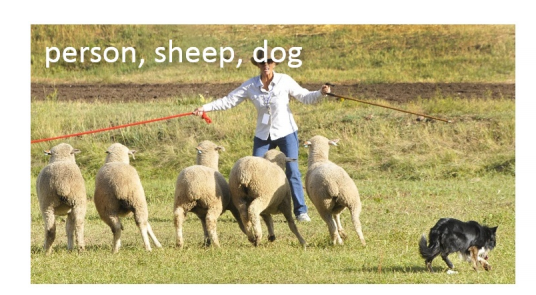
\includegraphics[width=\textwidth]{data_cls}
      \caption{}
      \label{fig:data_cls}
    \end{subfigure}%
    \qquad
    ~% add desired spacing
    \begin{subfigure}[b]{0.6\textwidth}
      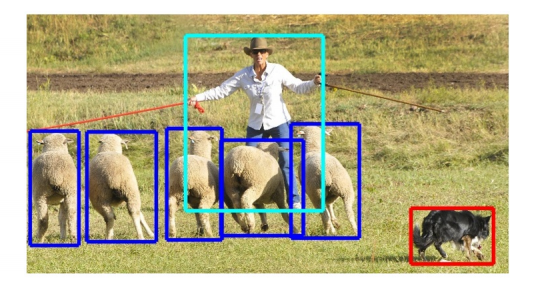
\includegraphics[width=\textwidth]{data_loc}
      \caption{}
      \label{fig:data_loc}
    \end{subfigure}
    \qquad
    \begin{subfigure}[c]{0.6\textwidth}
      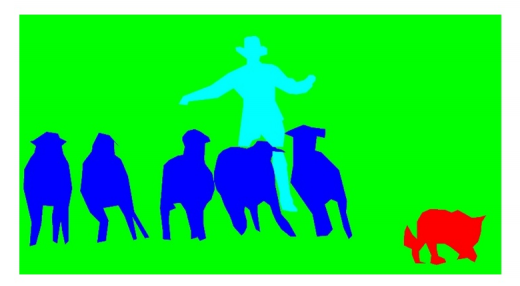
\includegraphics[width=\textwidth]{data_seg}
      \caption{}
      \label{fig:data_seg}
    \end{subfigure}

    \bicaption{计算机视觉主要任务(a)图片分类(b)物体检测(c)物体分割\cite{lin2014microsoft}}{Main tasks of computer vision(a)classification(b)detection(c)segmentation		\cite{lin2014microsoft}}
    \label{fig:dl_cv_task}
\end{figure}

一是分类(Classification),即是将图像结构化为某一类别的信息,用事先确定好的类别来对图片进行识别分类。这一任务是最简单、最基础的图像理解任务,也是深度学习模型最先取得突破和实现大规模应用的任务。其中,以ImageNet是评测集为代表的每年ILSVRC催生了大量的优秀深度网络结构,为其他任务提供了基础。在应用领域,人脸、场景等识别等都可以归为分类任务。

二是检测(Detection)。分类任务关心整体,给出的是整张图片的内容描述,而检测则关注特定的物体目标,要求同时获得这一目标的类别信息和位置信息。相比分类,检测给出的是对图片前景和背景的理解,需要从背景中分离出感兴趣的目标,并确定这一目标的描述(类别和位置),因而,检测模型的输出是一个列表,列表的每一项使用一个数据组给出检出目标的类别和位置(常用矩形检测框的坐标表示)。

三是分割(Segmentation)。分割包括语义分割(semantic segmentation)和实例分割(instance segmentation),前者是对前背景分离的拓展,要求分离开具有不同语义的图像部分,而后者是检测任务的拓展,要求描述出目标的轮廓(相比检测框更为精细)。分割是对图像的像素级描述,它赋予每个像素类别(实例)意义,适用于理解要求较高的场景,如无人驾驶中对道路和非道路的分割。

物体检测领域是CNN应用的相对较为广泛的项目,是本文主要采用的方法。检测模型整体上由基础网络和检测头部构成,前者作为特征提取器,给出图像不同大小、不同抽象层次的表示;后者则依据这些表示和监督信息学习类别和位置关联。检测头部负责的类别预测和位置回归两个任务常常是并行进行的,构成多任务的损失进行联合训练。

\subsection{两阶段物体检测模型}
两阶段物体检测模型因其对图片的两阶段处理得名,也称为基于区域(Region-based)的方法,其中又以R-CNN系列工作为这一系列的代表。
\begin{itemize}
	\item R-CNN\cite{40girshick2014rich}
	
	R-CNN(Regions with CNN features)作为R-CNN系列的开山之作,模型如图\ref{fig:dl_rcnn}所示。
	
	\begin{figure}[!htbp]
    \centering
    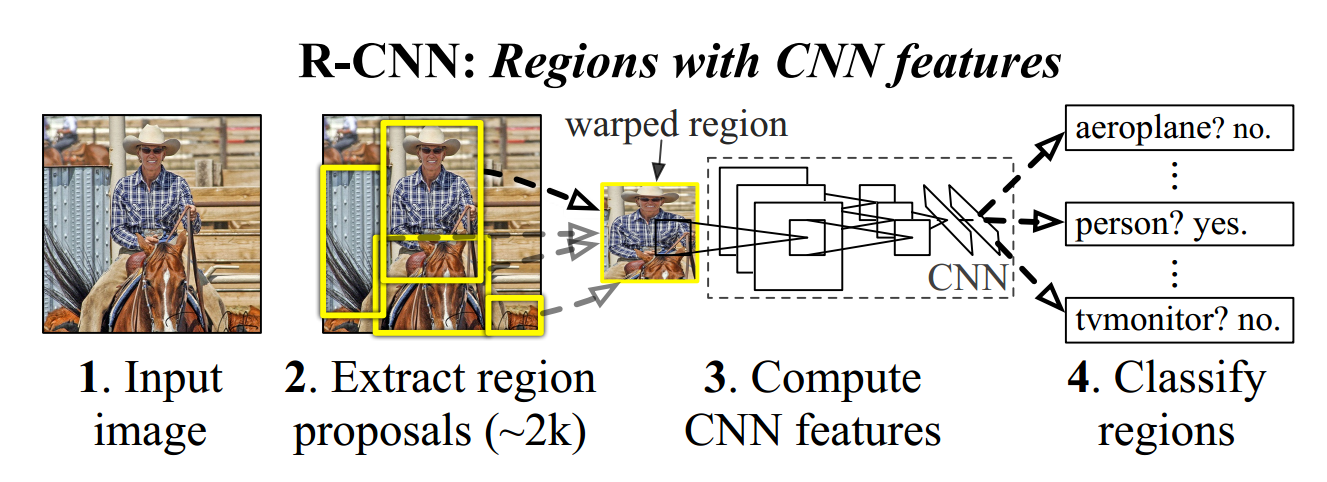
\includegraphics[width=1.0\textwidth]{dl_rcnn}
    \bicaption{R-CNN模型图\cite{40girshick2014rich}}{Architecture of R-CNN\cite{40girshick2014rich}}
    \label{fig:dl_rcnn}
	\end{figure}

R-CNN将检测抽象为两个过程,一是基于图片提出若干可能包含物体的区域(即图片的局部裁剪,被称为Region Proposal),文中使用的是Selective Search算法\cite{uijlings2013selective};二是在提出的这些区域上运行当时表现最好的分类网络(AlexNet)\cite{19krizhevsky2012imagenet},得到每个区域内物体的类别。R-CNN提出CNN可用于基于区域的定位和分割物体,而且当监督训练样本数紧缺时,在额外的数据上预训练的模型经过fine-tuning可以取得很好的效果。这种基于使用分类任务中中训练好的模型作为基网络,在检测问题上fine-tuning的做法一直被后面的两阶段模型所使用。模型本身存在的问题也很多,如需要训练三个不同的模型(Proposal,Classification,Regression)、重复计算过多导致的性能问题等。尽管如此,这篇论文的很多做法仍然广泛地影响着检测任务上的深度学习方法,后续的很多工作也都是针对改进这一工作而展开。

	\item Fast R-CNN\cite{41girshick2015fast}
	
	\begin{figure}[!htbp]
    \centering
    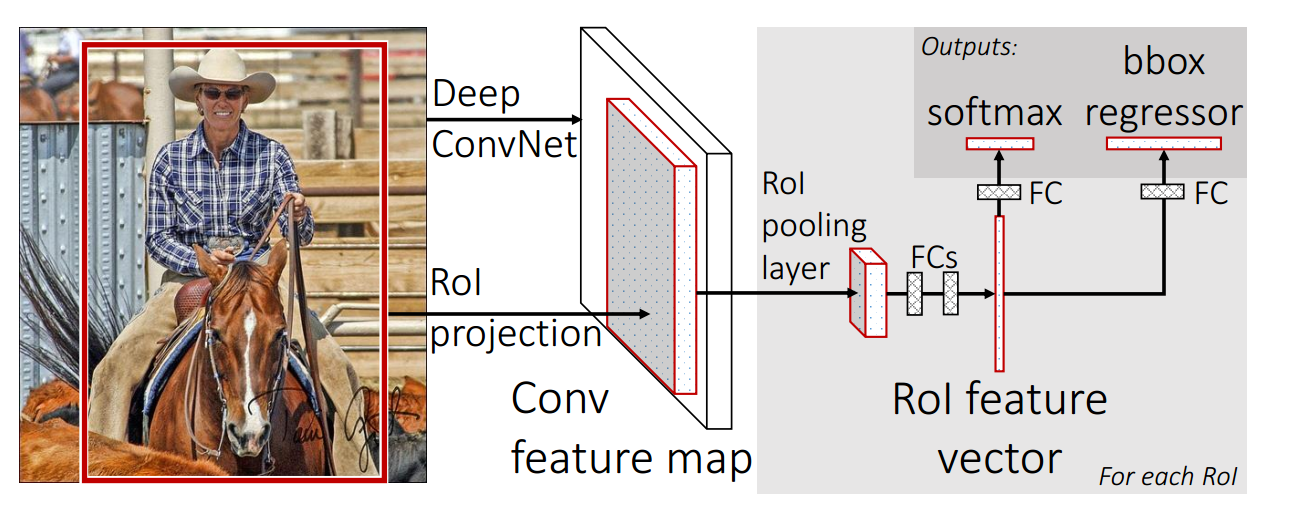
\includegraphics[width=1.0\textwidth]{dl_fastrcnn}
    \bicaption{Fast R-CNN模型图\cite{41girshick2015fast}}{Architecture of Fast R-CNN\cite{41girshick2015fast}}
    \label{fig:dl_fastrcnn}
	\end{figure}
	R-CNN耗时的原因是CNN是在每一个Proposal上单独进行的,没有共享计算,该模型将基础网络在图片整体上运行完毕后,再传入R-CNN子网络,共享了大部分计算,故有Fast之名。
	
	如图\ref{fig:dl_fastrcnn}是Fast R-CNN的架构图。图片经过feature extractor得到feature map, 同时在原图上运行Selective Search算法并将RoI(Region of Interset,实为坐标组,可与Region Proposal混用)映射到到feature map上,再对每个RoI进行RoI Pooling操作便得到等长的feature vector,将这些得到的feature vector进行正负样本的整理(保持一定的正负样本比例),传入并行的R-CNN子网络,进行分类和回归,并将两者的损失统一起来。
	
其中RoI Pooling是对输入R-CNN子网络的数据进行准备的关键操作。RPN得到的区域常常有不同的大小,在映射到feature map上之后,会得到不同大小的特征张量。RoI Pooling先将RoI等分成目标个数的网格,再在每个网格上进行max pooling,就得到等长的RoI feature vector。文章将Proposal,Feature Extractor,Object Classification和Localization统一在一个整体的结构中,并通过共享卷积计算提高特征利用效率,是最有贡献的地方。
	
	\item Faster R-CNN\cite{30ren2015faster}
	
	Faster R-CNN是2-stage方法的奠基性工作,提出的RPN网络取代Selective Search算法使得检测任务可以由神经网络端到端地完成。粗略的讲,Faster R-CNN = RPN + Fast R-CNN,跟R-CNN共享卷积计算的特性使得RPN引入的计算量很小,使得Faster R-CNN可以在单个GPU上以5fps的速度运行,而在精度方面达到SOTA(State of the Art,当前最佳)。
	
Faster R-CNN的主要贡献是提出Regional Proposal Networks,替代之前的Selective Search算法。RPN网络将Proposal这一任务建模为二分类(是否为物体)的问题。

	\begin{figure}[!htbp]
    \centering
    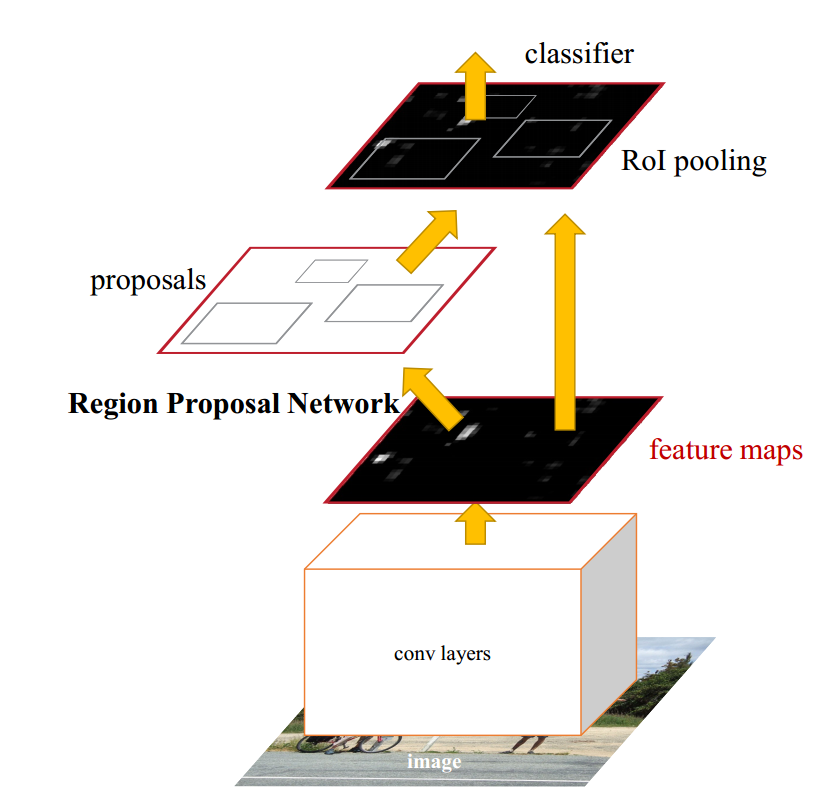
\includegraphics[width=0.7\textwidth]{dl_rpn}
    \bicaption{RPN模型\cite{30ren2015faster}}{Architecture of RPN\cite{30ren2015faster}}
    \label{fig:dl_rpn}
	\end{figure}
	如图\ref{fig:dl_rpn}第一步是在一个滑动窗口上生成不同尺寸(scales)和长宽比例(aspect ratio)的anchor box,取定IoU的阈值,按ground-truth标定这些anchor box的正负。于是,传入RPN网络的样本数据被整理为anchor box(坐标)和每个anchor box是否有物体(二分类标签)。RPN网络将每个样本映射为一个概率值和四个坐标值,概率值反应这个anchor box有物体的概率,四个坐标值用于回归定义物体的位置。最后将二分类和坐标回归的损失统一起来,作为RPN网络的目标训练。
	
由RPN得到Region Proposal在根据概率值筛选后经过类似的标记过程,被传入R-CNN子网络,进行多分类和坐标回归,同样用多任务损失将二者的损失联合。

遵循multi-task loss定义,最小化目标函数,Faster R-CNN中对一个图像的损失函数定义为:

\begin{equation}
	L\left(\left\{p_{i}\right\},\left\{u_{i}\right\}\right)=\frac{1}{N_{c l s}} \sum_{i} L_{cls}\left(p_{i}, p_{i}^{*}\right)+\lambda \frac{1}{N_{r e g}} \sum_{i} p_{i}^{*} L_{r e g}\left(t_{i}, t_{i}^{*}\right)
\end{equation}

这个可以考虑为从anchor box回归到附近的ground-truth box。其中$p_i$为anchor预测为目标的概率,GT标签:$p_{i}^{*}=\left\{\begin{array}{ll}{0} & {\text { negative label }} \\ {1} & {\text { positive label }}\end{array}\right., \quad t_{\mathrm{i}}=\left\{t_{x}, t_{y}, t_{w}, t_{h}\right\}$一个向量,表示预测的boungding box包围盒的4个参数化坐标,$t_{i}^{*}$是与positive anchor对应的ground-truth包围盒的坐标向量,具体计算如下:

\begin{equation}
	\begin{aligned} t_{\mathrm{x}} &=\left(x-x_{a}\right) / w_{a} ; t_{y}=\left(y-y_{a}\right) / h_{a} \\ t_{\mathrm{w}} &=\log \left(w / w_{a}\right) ; t_{h}=\log \left(h / h_{a}\right) \\ t_{x}^{*} &=\left(x-x_{a}\right) / w_{a} ; t_{y}^{*}=\left(y^{*}-y_{a}\right) / h_{a} \\ t_{w}^{*} &=\log \left(w^{*} / w_{a}\right) ; t_{h}^{*}=\log \left(h^{*} / h_{a}\right) \end{aligned}
\end{equation}

$L_{c l s}\left(p_{i}, p_{i}^{*}\right)$是两个类别(目标vs非目标)之间的对数损失,为交叉熵损失函数,计算如下:
\begin{equation}
	L_{c l s}\left(p_{i}, p_{i}^{*}\right)=-\log \left[p_{i}^{*} p_{i}+\left(1-p_{i}^{*}\right)\left(1-p_{i}\right)\right]
\end{equation}

$L_{r e g}\left(t_{i}, t_{i}^{*}\right)$是回归损失函数,计算如下:
\begin{equation}
	L_{r e g}\left(t_{i}, t_{i}^{*}\right)=R\left(t_{i}-t_{i}^{*}\right)
\end{equation}

其中R是smooth L1损失函数。
$p_{i}^{*} L_{r e g}$表示只有前景anchor$\left(p_{i}^{*}=1\right)$才有回归损失,其他情况则没有。cls层和reg层的输出分别由$\left\{p_{i}\right\},\{u\}$控制,这两项分别由$N_{c l s}$和$N_{\text {reg}}$以及一个平衡权重$\lambda$归一化。

Faster R-CNN的成功之处在于用RPN网络完成了检测任务的深度化。使用滑动窗口生成anchor box的思想也在后来的工作中越来越多地被采用。这项工作奠定了RPN+RCNN的两阶段结构,影响了大部分后续工作。

\end{itemize}

\subsection{单阶段物体检测模型}
\begin{itemize}
	\item YOLO\cite{32redmon2016you}
	\begin{figure}[!htbp]
    \centering
    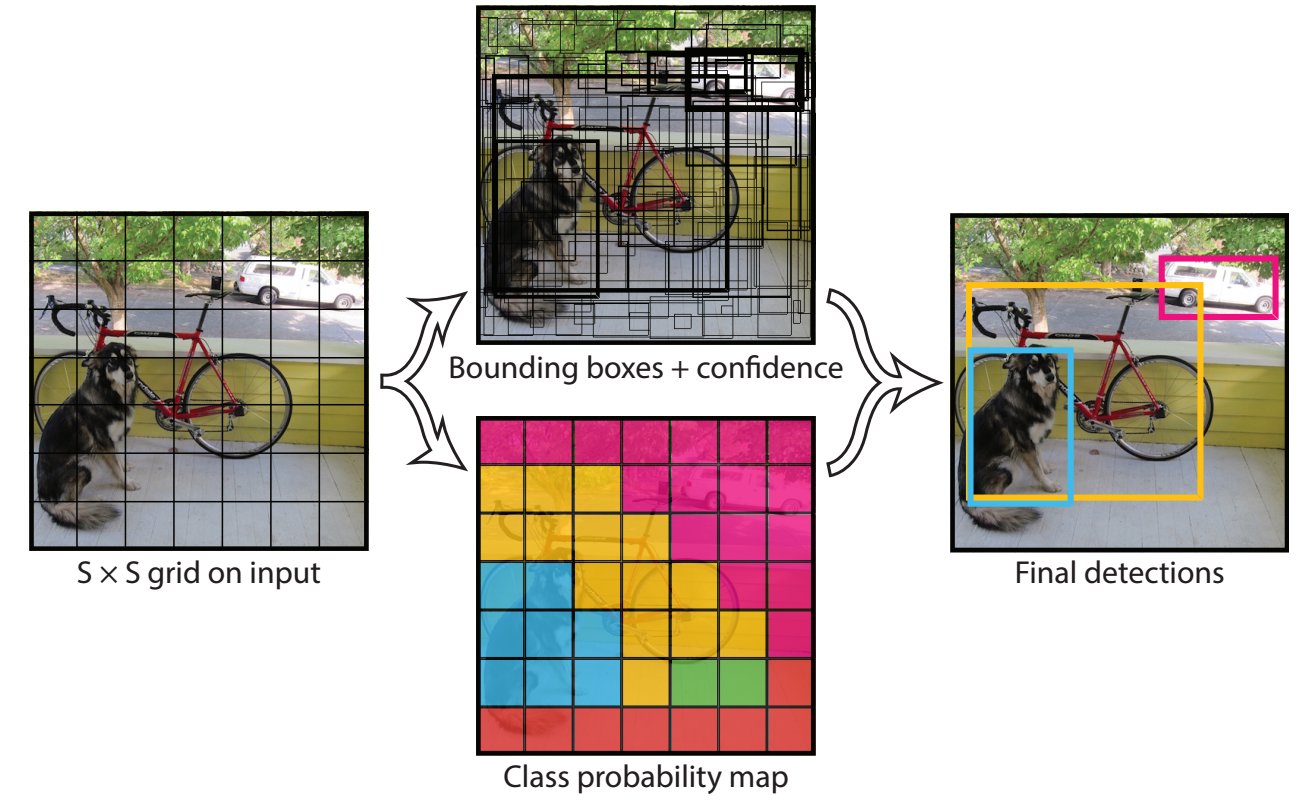
\includegraphics[width=1.0\textwidth]{dl_yolo}
    \bicaption{YOLO模型\cite{32redmon2016you}}{Architecture of YOLO\cite{32redmon2016you}}
    \label{fig:dl_yolo}
	\end{figure}
	如图\ref{fig:dl_yolo}YOLO的工作流程如下:
	
1.准备数据:将图片缩放,划分为等分的网格,每个网格按跟ground-truth的IoU分配到所要预测的样本。

2.卷积网络:由GoogLeNet\cite{szegedy2015going}更改而来,每个网格对每个类别预测一个条件概率值,并在网格基础上生成B个box,每个box预测五个回归值,四个表征位置,第五个表征这个box含有物体(不是某一类物体)的概率和位置的准确程度(由IoU表示)。测试时,分数如下计算:
\begin{equation}
	\operatorname{Pr}\left(\text {Class}_{i} | \text { Object }\right)^{*} \operatorname{Pr}(\text {Object})^{*} \text{IOU}_{pred}^{truth}=\operatorname{Pr}\left(\text {Class}_{i}\right)^{*} \text{IOU}_{pred}^{truth}
\end{equation}

等式左边第一项由网格预测,后两项由每个box预测,以条件概率的方式得到每个box含有不同类别物体的分数。 因而,卷积网络共输出的预测值个数为S×S×(B×5+C),其中S为网格数,B为每个网格生成box个数,C为类别数。

3. 后处理:使用NMS(Non-Maximum Suppression,非极大抑制)\cite{hosang2017learning}过滤得到最后的预测框

非极大值抑制的方法是:先假设有6个矩形框,根据分类器的类别分类概率做排序,假设从小到大属于车辆的概率分别为A、B、C、D、E、F。
\begin{itemize}
	\item 从最大概率矩形框F开始,分别判断A、E与F的重叠度IOU是否大于某个设定的阈值。
	\item 假设B、D与F的重叠度超过阈值,那么就扔掉B、D;并标记第一个矩形框F,是保留下来的。
	\item 从剩下的矩形框A、C、E中,选择概率最大的E,然后判断E与A、C的重叠度,重叠度大于一定的阈值,那么就扔掉;并标记E是保留下来的第二个矩形框。
	就这样一直重复,找到所有被保留下来的矩形框。
\end{itemize}


损失函数被分为三部分:坐标误差、物体误差、类别误差。为了平衡类别不均衡和大小物体等带来的影响,损失函数中添加了权重并将长宽取根号。YOLO提出了单阶段的新思路,相比两阶段方法,其速度优势明显,同时可以实时检测。但YOLO本身也存在一些问题,如划分网格较为粗糙,每个网格生成的box个数等限制了对小尺度物体和相近物体的检测。

	\item SSD\cite{37Liu2016SSD}
	
	如图\ref{fig:dl_ssd},SSD(Single Shot Detector)相比YOLO有以下突出的特点:
		\begin{figure}[!htbp]
    \centering
    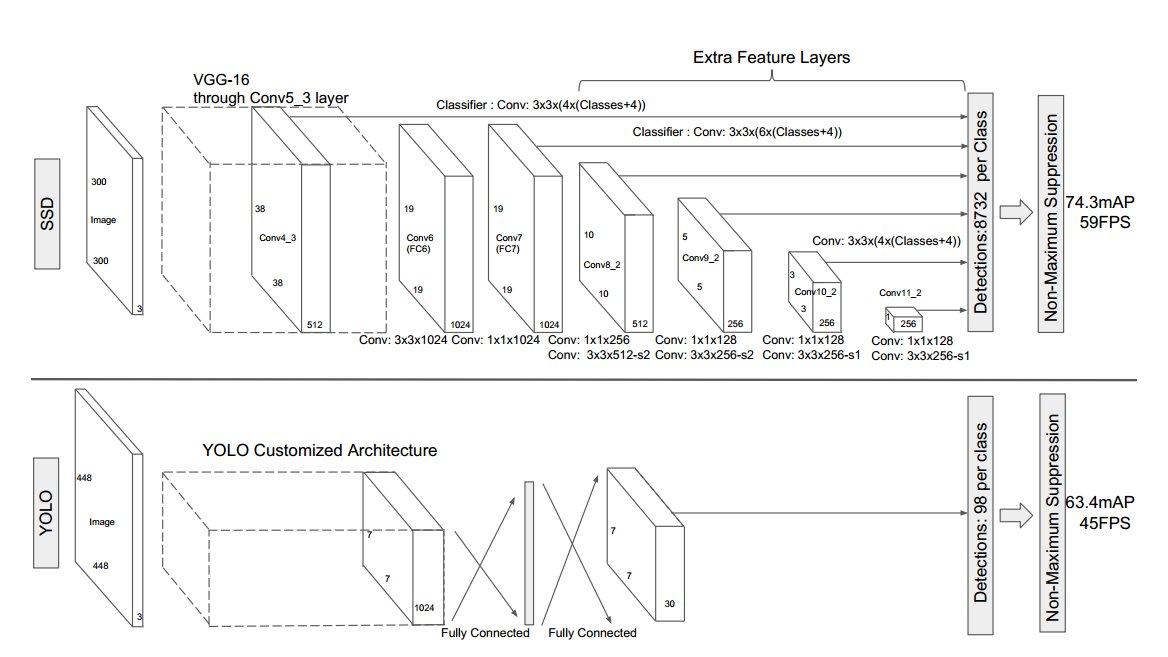
\includegraphics[width=1.0\textwidth]{dl_ssd}
    \bicaption{SSD模型\cite{37Liu2016SSD}}{Architecture of SSD\cite{37Liu2016SSD}}
    \label{fig:dl_ssd}
	\end{figure}
	\begin{itemize}
		\item 多尺度的feature map:基于VGG的不同卷积段,输出feature map到回归器中。这一点试图提升小物体的检测精度。
		\item 更多的anchor box,每个网格点生成不同大小和长宽比例的box,并将类别预测概率基于box预测(YOLO是在网格上),得到的输出值个数为(C+4)×k×m×n,其中C为类别数,k为box个数,m×n为feature map的大小。
		
	\end{itemize}
	
	SSD是单阶段模型早期的集大成者,达到跟接近两阶段模型精度的同时,拥有比两阶段模型快一个数量级的速度。后续的单阶段模型工作大多基于SSD改进展开。	
\end{itemize}
\section{迁移学习}

在传统计算机视觉领域,由于图片标注成本小,数据量往往不是一个主要的问题。而对于医学影像,存在需要专业医生标注,数据获取困难等问题,针对现有的少量数据集进行研究就成为核心问题。如图\ref{fig:dl_tl},迁移学习(Transfer learning)\cite{63pan2010survey}就是把已学训练好的模型参数迁移到新的模型来帮助新模型训练。考虑到大部分数据或任务是存在相关性的,所以通过迁移学习可以将已经学到的模型参数(也可理解为模型学到的知识)通过某种方式来分享给新模型从而加快并优化模型的学习效率不用像大多数网络那样从零学习。其初衷是节省人工标注样本的时间,让模型可以通过已有的标记数据(source domain data)向未标记数据(target domain data)迁移,从而训练出适用于target domain的模型。

迁移学习按照学习方式可以分为基于样本的迁移,基于特征的迁移,基于模型的迁移,以及基于关系的迁移。基于样本的迁移通过对源域中有标定样本的加权利用完成知识迁移;基于特征的迁移通过将源域和目标域映射到相同的空间(或者将其中之一映射到另一个的空间中)并最小化源域和目标域的距离来完成知识迁移;基于模型的迁移将源域和目标域的模型与样本结合起来调整模型的参数;基于关系的迁移则通过在源域中学习概念之间的关系,然后将其类比到目标域中,完成知识的迁移。
	\begin{figure}[!htbp]
    \centering
    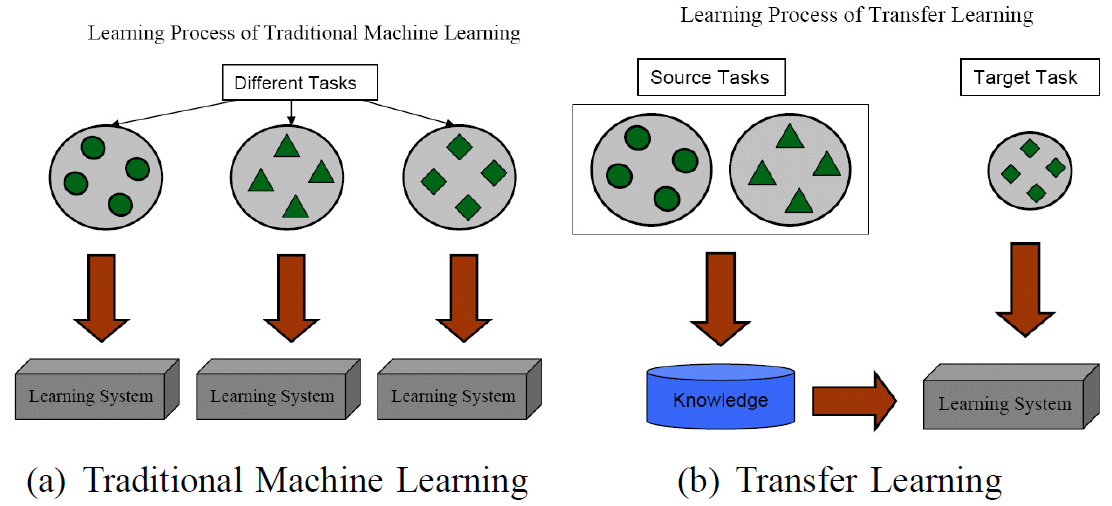
\includegraphics[width=1.0\textwidth]{dl_tl}
    \bicaption{迁移学习与传统机器学习的不同。(a)传统机器学习对不同的学习任务建立不同的模型,(b)迁移学习利用源域中的数据将知识迁移到目标域,完成模型建立。}{The difference between Migration learning and traditional machine learning. (a) Traditional machine learning establishes different models for different learning tasks. (b) Migration learning uses data from the source domain to migrate knowledge to the target domain and complete model building.}
    \label{fig:dl_tl}
	\end{figure}
	主要的迁移学习方法如下:
	\begin{itemize}
		\item ConvNet固定特征提取器
		
		取出ImageNet ConvNet预训练好的模型,移除最后一个全连接层(该层的输出是一个不同的任务,如ImageNet 1000级评分),然后把剩下的ConvNet作为新数据集的固定特征提取器。模型将计算每个图像包含的激活层之前的隐藏层所提取出来的特征,之后将特征放入一个线性分类器(如线性SVM和softmax分类器)进行分类从而得到最终的结果。在乳腺钼靶图片的小数据集上,可以采用在传统深度学习模型上固定相关层从而获取浅层特征,进而将获取到的浅层特征与深层特征进行连接重新进行训练,从而得到最终分类结果。
		
		\item 微调ConvNet
		
		在新的数据集上,这种策略不仅是要更换和重训练ConvNet的顶层结构,也需要微调网络中训练出来的网络权重。可能微调ConvNet的所有层,或把之前的一些层固定是可能的(由于过度拟合问题)只是微调一些网络的顶层部分。ConvNet早期特征中包含更多的一般特征(如边缘检测、彩色斑点探测器)应该是许多任务有用,但ConvNet的顶层部分由于细节越来越具体,使得在新数据集上并不完全适应。
		
	\end{itemize}

迁移学习一般要考虑的图片分为几种情况。数据集小并且类似于原有数据集,数据集大而且类似于原有数据集,数据集小但和原有数据集差别大,数据集大但和原有数据集差别大。

对于乳腺钼靶图片问题,数据与传统的计算机视觉数据集差别大,而且数据量小,这属于迁移学习中最难的问题,由于特征之间差别小,所以使用固化顶层模块来训练模型就变得不再有效,需要针对此问题要么提升特征提取器的能力,要么设计全新的模块或损失函数。 

\section{弱监督学习}
机器学习在各种任务中取得了巨大成功,特别是在分类和回归等监督学习任务中。预测模型是从包含大量训练样本的训练数据集中学习,每个训练样本对应一个事件或对象。训练样本由两部分组成:一个描述事件/对象的特征向量(或示例),以及一个表示真值输出的标签。在分类任务中,标签表示训练样本所属的类别;在回归任务中,标签是一个与样本对应的实数值。大多数成功的技术,如深度学习,都需要含有真值标签的大规模训练数据集,监督学习技术在具备强监督信息(如大量具备真值标签的训练样本)的情况中取得了很大成功。总的来说,监督学习就是正常用的,有一批高置信的标注数据,通过模型来拟合效果。然而,在许多任务中,由于数据标注过程的成本极高,很难获得强监督信息,因此,使用弱监督学习通常是更好的方式。弱监督学习\cite{43zhou2017brief},就是很难获取足够量的高置信的标注数据,所以弱监督学习就是来解决这个问题。

通常来说,弱监督可以分为三类。第一类是不完全监督(incomplete supervision),即只有训练集的一个(通常很小的)子集是有标签的,其他数据则没有标签。这种情况发生在各类任务中。例如,在图像分类任务中,真值标签由人类标注者给出的。从互联网上获取巨量图片很容易,然而考虑到标记的人工成本,只有一个小子集的图像能够被标注。第二类是不确切监督(inexact supervision),即图像只有粗粒度的标签。第三种是不准确的监督(inaccurate supervision),模型给出的标签不总是真值。出现这种情况的常见原因有,图片标注者不小心或比较疲倦,或者某些图片就是难以分类。

弱监督方法常见的步骤先是利用监督信息训练,之后去人为预测未监督信息,使其带有人为的标签,然后再次重点去识别分类二者区别。而这也是乳腺钼靶整图分类的常见做法,获取可以病灶区域patch,进而进行再次细致识别。
本文的数据属于给定了监督信息,但信息不够精确的场景,对于物体检测问题而言,同时拥有标注和分类信息才是模型能否学习充分的关键,然而该项目存在只有恶性数据含有标注信息,而正常数据没有标注信息的问题,所以在进行模型具体设计时,需要引入这种弱监督学习的方法。

\begin{comment}
\section{多示例学习}
不确切监督关注于给定了监督信息,但信息不够精确的场景。一个典型的场景是仅有粗粒度的标签信息可用。例如,在药物活性预测\cite{44dietterich1997solving}的问题中,其目标是建立一个模型学习已知分子的知识,来预测一个新的分子是否适合制造一种特定药物。一个分子可以有很多的低能量形状,而这些分子是否能用于制药取决于这些分子是否具有某些特殊的形状。然而即使对于已知的分子,人类专家也仅知道该分子是否适合制药,而不知道其中决定性的分子形状是什么。形式化表达为,该任务是从训练数据集$D=\left\{\left(X_{1}, y_{1}\right), \ldots,\left(X_{m}, y_{m}\right)\right\}$中学习$f : \chi \mapsto \gamma$
,其中$X_{i}=\left\{x_{i 1}, \ldots, x_{i, m_{i}}\right\} \subseteq \chi$被称为一个包。 $x_{i j} \in \chi\left(j \in\left\{1, \ldots, m_{i}\right\}\right)$是一个示例, $m_{i}$是示例 $X_{i}$的数量,$y_{i} \in \gamma=\{Y, N\}$, $X_{i}$是一个 positive包,即$y_{i}=Y$,如果存在$X_{i}$是正的,同时$p \in\left\{1, \ldots, m_{i}\right\}$是未知的。其目标是为未见过的包预测标签。该方法被称为多示例学习\cite{45foulds2010review}。
 
已经有许多有效的算法被开发出来并应用于多示例学习。实际上,几乎所有的有监督学习算法都有对等的多示例算法。大多数算法试图调整单示例监督学习算法,使其适配多示例表示,主要是将其关注点从对示例的识别转移到对包的识别\cite{46zhou2006multi};一些其他算法试图通过表示变换,调整多示例表示使其适配单示例算法\cite{47zhou2007solving}。还有一种类型\cite{48amores2013multiple},将算法分为三类:一个整合了示例级响应的示例空间范式,一个把包视作一个整体的包空间范式,以及一个在嵌入特征空间中进行学习的嵌入空间范式中。这些示例通常被视为独立同分布样本,然而,\cite{49zhou2007relation}表明,多示例学习中的示例不应该被认为是独立的,尽管这些包可以被视为独立同分布样本,并且已经有一些有效的算法是基于此见解进行开发的\cite{50zhou2009multi}。

多示例学习已成功应用于各种任务,如图像分类/检索/注释\cite{51chen2004image, 52zhang2002content, 53tang2010image},医学诊断\cite{54dundar2007multiple},面部/对象检测\cite{55zhang2006multiple, 56felzenszwalb2010object},对象类别发现\cite{57zhu2015unsupervised},对象跟踪\cite{58zhu2015unsupervised}等。在这些任务中,将真实对象(例如一幅图像或一个文本文档)视为一个包是很自然的。然而,不同于药物活性预测这类包中包含天然示例(分子的各种形状)的例子,需要为每个包生成示例。包生成器制定如何生成示例来构成包。通常情况下,可以从图像中提取许多小的图像块作为其示例,而章节/段落甚至句子可以用作文本文档的示例。

多示例学习的初始目标是为未见过的包预测标签;然而,已有研究尝试识别那些之所以让正包变正的关键示例(key instance)。这在诸如没有细粒度标记训练数据的感兴趣区域定位的任务中特别有用。值得注意的是,标准的多示例学习 \cite{59dietterich1997solving}假定每一个正包必须包含一个关键示例,而还有其它研究假定不存在关键示例,每一个示例都对包标签有贡献\cite{60xu2004logistic, 61chen2006miles};甚至假定存在多个概念,而仅当一个包包含满足所有概念的示例时,该包才是正的。

本文由于考虑的数据存在多层面的问题,除了在基于图片标准可以按照传统的标准来制定之外,考虑单个乳房,单个病例情况都需要引入多示例学习对结果进行评判。
\end{comment}

\section{度量学习}
度量学习 (Metric Learning)\cite{65bellet2013survey},更确切地可以说是距离度量学习 (Distance Metric Learning,DML)、相似度学习。度量学习是人脸识别中常用传统机器学习方法,由Eric Xing在NIPS 2002提出。分为两种,一种是基于监督学习的,另外一种是基于非监督学习的,根据不同的任务来自主学习出针对某个特定任务的度量距离函数。通过计算两张图片之间的相似度,使得输入图片被归入到相似度大的图片类别中去,其中以孪生网络最为著名。

孪生网络(Siamese network)\cite{42chopra2005learning}是一种网络结构,通过一个神经网络将样本的维度降低到某个较低的维度。

在低维空间,任意两个样本:
\begin{itemize}
	\item 如果它们是相同类别,空间距离尽量接近0;
	\item 如果它们是不同类别,空间距离大于某个间隔。
	
\end{itemize}

Siamese network就是“连体的神经网络”,神经网络的“连体”是通过共享权值来实现的,如图\ref{fig:dl_simnet}所示。

	\begin{figure}[!htbp]
    \centering
    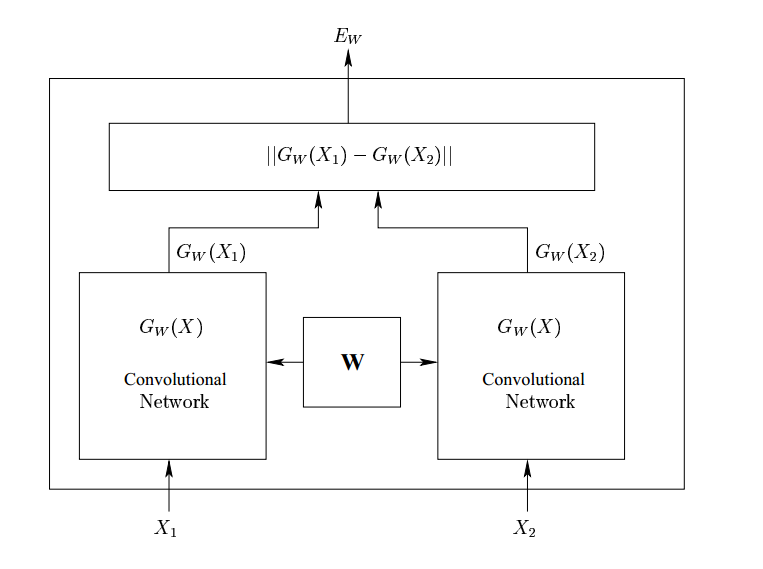
\includegraphics[width=0.7\textwidth]{dl_simnet}
    \bicaption{孪生网络图\cite{42chopra2005learning}}{Architecture of Siamese network\cite{42chopra2005learning}}
    \label{fig:dl_simnet}
	\end{figure}

孪生网络的目的是为了比较两幅图片是否相似,或者说相似度多少。输入是两张需要对比的图片,输出则是一个相似度数值。孪生网络现在越来越广泛应用于人脸识别,图像块匹配,跟踪等问题,并在此基础上改进和更新了诸多模块和损失函数。Siamese network的初衷是计算两个输入的相似度,左右两个神经网络分别将输入转换成一个“向量”,在新的空间中,通过判断cosine距离就能得到相似度。cosine、exp function、欧式距离均可以作为相似度距离。模型训练的目标是让两个相同的输入距离尽可能的小,两个不同类别的输入距离尽可能的大。根据实验分析,cosine更适用于词汇级别的语义相似度度量,而exp更适用于句子级别、段落级别的文本相似性度量。

在本文中,由于需要模型去区分疑似的恶性病灶和恶性病灶之间的区别,所以需要引入孪生网络设计思想及其损失函数。

\section{本章小结}
本章在对数据进行充分分析的情况下,具体介绍了本文所使用到的相关深度学习技术,包括卷积神经网络、基于CNN的物体检测模型、迁移学习、弱监督学习和度量学习等,为后续项目的开展提供理论支持。